\documentclass{mylib/reporteConCalif}

\usepackage{tabu}

\title{Reporte}
\author{rodrigofranciscopablo }

\subject{Laboratorio de Dispositivos y circuitos electrónicos}
\mytitle{Reporte de práctica 3}
\mysubTitle{El diodo semiconductor y Zener}
\students{Francisco Pablo \textsc{Rodrigo}}
\teacher{M.I. Guevara Rodríguez \textsc{Ma. del Socorro}}
\group{8}
\deliverDate{6 de marzo de 2019}

\newcommand{\funx}{x_1(a,b,c,d) = [a \cdot \overline{b}(c+b \cdot d) + \overline{a} \cdot \overline{b} ]c}

\begin{document}

\coverPage

%\tableofcontents
%\newpage

\section*{Desarrollo}

\subsection*{Diodo rectificador con polarización directa}
\begin{center}
	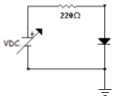
\includegraphics[scale=1]{img/labdisp_pract3/diodorec_d}


	\begin{tabu} to 0.8\textwidth { | X[c] | X[c] | X[c] | X[c] | X[c] | X[c] | X[c] | X[c] | X[c] | }
	 \hline
	 $I_{D}$ & $10 \mu A$ & $50 \mu A$ & $100 \mu A$ & $500 \mu A$ & $1 mA$ & $10 mA$ & $20 mA$ & $30 mA$\\
	 \hline
	 $V_{D_{teo}}$ & $0 mV$ & $0.5 mV$ & $0.53 mV$ & $0.59 mV$ & $0.62 mV$ & $0.7 mV$ & $0.73 mV$ & $0.74 mV$\\
	\hline
	$V_{D_{prac}}$ & $0 mV$ & $0.52 mV$ & $0.55 mV$ & $0.60 mV$ & $0.66 mV$ & $0.74 mV$ & $0.76 mV$ & $0.79 mV$\\
	\hline
	\end{tabu}

\end{center}

Podemos observar que los valores de voltaje teórico y práctico no difieren en mucho por lo que podemos concluir que la gráfica mostrada en el \textbf{Previo} es correcta.

\subsection*{Diodo rectificador con polarización inversa}
\begin{center}
	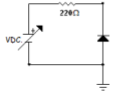
\includegraphics[scale=1]{img/labdisp_pract3/diodorec_i}


	\begin{tabu} to 0.8\textwidth { | X[c] | X[c] | X[c] | X[c] | X[c] | X[c] | X[c] |  }
	 \hline
	 $I_{D}$ & $1 \mu A$ & $5 \mu A$ & $10 \mu A$ & $15 \mu A$ & $20 \mu A$ & $25 \mu A$ \\
	 \hline
	 $V_{D_{teo}}$ & $50 mV$ & $50.1 mV$ & $50.2 mV$ & $50.2 mV$ & $50.2 mV$ & $50.2 mV$ \\
	\hline
	 $V_{D_{prac}}$ & $0 mV$ & $0 mV$ & $0 mV$ & $0 mV$ & $0 mV$ & $0 mV$ \\
	\hline
	\end{tabu}

\end{center}

En este caso los valores difieron terriblemente ya que en la vida real un rectificador con polarización inversa no debe dejar pasar corriente.

\subsection*{Diodo Zener con polarización directa}
\begin{center}
	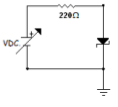
\includegraphics[scale=1]{img/labdisp_pract3/diodoz_d}


	\begin{tabu} to 0.8\textwidth { | X[c] | X[c] | X[c] | X[c] | X[c] | X[c] | X[c] | X[c] | X[c] | }
	 \hline
	 $I_{D}$ & $10 \mu A$ & $50 \mu A$ & $100 \mu A$ & $500 \mu A$ & $1 mA$ & $10 mA$ & $20 mA$ & $30 mA$\\
	 \hline
	 $V_{D_{teo}}$ & $0.18 mV$ & $0.22 mV$ & $0.24 mV$ & $0.28 mV$ & $0.30 mV$ & $0.41 mV$ & $0.47 mV$ & $0.54 mV$\\
	\hline
	$V_{D_{prac}}$ & $0.20 mV$ & $0.23 mV$ & $0.25 mV$ & $0.29 mV$ & $0.31 mV$ & $0.42 mV$ & $0.49 mV$ & $0.60 mV$\\
	\hline
	\end{tabu}

\end{center}



\subsection*{Diodo rectificador con polarización inversa}
\begin{center}
	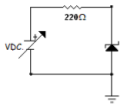
\includegraphics[scale=1]{img/labdisp_pract3/diodoz_i}


	\begin{tabu} to 0.8\textwidth { | X[c] | X[c] | X[c] | X[c] | X[c] | X[c] | X[c] |  }
	 \hline
	 $I_{D}$ & $1 \mu A$ & $5 \mu A$ & $10 \mu A$ & $15 \mu A$ & $20 \mu A$ & $25 \mu A$ \\
	 \hline
	 $V_{D_{teo}}$ & $4.82 mV$ & $4.86 mV$ & $4.88 mV$ & $4.89 mV$ & $4.90 mV$ & $4.9 mV$ \\
	\hline
	$V_{D_{prac}}$ & $4.90 mV$ & $4.92 mV$ & $4.94 mV$ & $4.95 mV$ & $4.98 mV$ & $5.3 mV$ \\
	\hline
	\end{tabu}

\end{center}

Para el caso de del diodo Zener hay que recordar que este dispositivo conduce la corriente en ambos sentidos solo que debemos de tener cuidado pues el voltaje del diodo en polarización directa es el mismo que en polarización inversa.


\section*{Conclusiones}

Tanto el diodo semiconductor como el diodo Zener tienen sus aplicaciones y su importancia para el uso de dispositivos electrónicos. Observando las curvas de cada uno, podemos observar su comportamiento y vemos que, por ejemplo, para el diodo semiconductor, vimos que dependiendo la polaridad en la que estuviera conectado, dejaba que hubiera flujo o no de corriente eléctrica, y eso se comprobó con el foco que conectamos, ya que con polaridad abierta, la corriente circulaba y se prendía el foco, y con polaridad cerrada, había corriente pero no llegaba hasta el foco, por lo tanto, no se enciende.

\end{document}